\documentclass[11pt]{article}

\usepackage{framed}
\usepackage{float}
\usepackage{listings}
\usepackage{graphicx}

\begin{document}
	\title{\texttt{markov\_populator.py} Documentation}
	\date{\today}
	\maketitle
	
	\section{Introduction}
	This document serves to explain the algorithm behind how the script
	\texttt{markov\_populator.py} functions and how a user may use it to produce
	scenarios.  This script lives within the \texttt{GOSM} library and the
	proper installation of the most recent version of \texttt{GOSM} will 	
	correctly install this script. Note it may be necessary to run
	\texttt{python setup.py install} again if you do not have the most recent
	version installed.
	
	\section{Algorithm}
	This section will serve as a brief description how the script actually
	produces scenarios. It functions by first classifying given historic data on
	forecasts, actuals, and errors, each historic date-time into a specific
	state $S_i$. The state will generally just be an interval that a certain 
	field is in. For example if we have that the error at a given time is 125, 
	then the corresponding state might be $[100, 150]$. It might also be
	preferred to specify the state by quantiles in which case the state might be
	$[0.2,0.4]$. In the simplest case, the state will just be an error interval,
	but in separate tests, it may be useful to include the forecast interval or
	the forecast derivative interval in the state.
	Then given this mapping of date-times to states produces a 
	transition matrix $A$ where $A_{ij}$ is the frequency with which state 
	$S_j$ follows state $S_i$. Empirically we take this as the probability with
	which one state will proceed another. 
	
	For each scenario on a specific day, we choose a start state for the Markov 
	Chain. To do this, we categorize the first hour of that day based on the 
	forecast into a certain state and pick a random sample from the historically
	observed states which fall into the same forecast category. Then using this
	start state, we transition from state to state based on the probabilities in
	the transition matrix until we have a state for all 24 hours of the day.
	
	Using this sequence of states, we then can convert this into an 24-error 
	vector by sampling from an empirical distribution on the error interval of
	the state. This error is then added to the daily forecast which then is
	truncated at 0 and the capacity of the source to complete the scenario.
	
	\section{Input Files}
	This script only requires two input files, a data file and an options file.
	The data file is structured the same as is used for \texttt{prescient} and
	is described here for good measure.
	These files are described in turn.
	
	Once you have both of these, with an appropriately structured options file,
	the script can be executed with the command:
	\begin{verbatim}
		runner.py <options_file>
	\end{verbatim}
	where \texttt{<options\_file>} is replaced by the name of the file.
	
	\input{data.tex}
		
	\subsection{Options File}
	The options file specifies how you may configure behavior of the script to
	generate scenarios differently. Any option's description can be found using 
	the command \texttt{python markov\_populator.py -h}. We discuss the most
	common options here. We begin by presenting the most basic
	example of an options file in Figure \ref{example1}.
	
	\begin{figure}[H]
	\begin{framed}
		\lstinputlisting{markov_example1.txt}
	\end{framed}
	\label{example1}
	\caption{A basic example of an options file}
	\end{figure}
	
	The first thing we note is that all options file used for executing this
	script must begin with the following line verbatim:
	\begin{verbatim}
		command/exec markov_populator.py
	\end{verbatim}
	This specifies to the script \texttt{runner.py} which program to actually
	run.
	
	Also contained in this script are required options for every run of 
	\texttt{markov\_populator.py}. Namely, these are \texttt{--power-source}
	which specifies the data file which contains forecasts and actuals, 
	\texttt{--start-date} and \texttt{--end-date} which specify the date range
	for which you would like to produce scenarios, and 
	\texttt{--output-directory} which specifies where to store all the output
	files.
	
	In addition, this specifies the number of scenarios to generate with the 
	\texttt{--number-of-scenarios} option. All other options are left to
	defaults. This means that the exact specification for what a state is
	will simply be which interval the recorded error is in. Put more precisely,
	the separate error states will be intervals of length 100 and the entire
	set is given by $\{[0, 100], [100, 200], \ldots\}$. This specific length
	can be adjusted with the \texttt{--error-bin-size} argument. Note that the
	limits of the intervals will always be multiples of this size option.
	
	An example where the user expresses more control over the what a state
	actually is can be seen in Figure \ref{example2}. Note that here, the user
	specifies that they would like to use quantile intervals instead of raw
	energy intervals with the \texttt{--use-error-quantiles} option. The user
	also specifies the exact width of the intervals with the 
	\texttt{--error-quantile-size} option. This means the states will 
	be quantile intervals $\{[0,0.1],[0.1,0.2],\ldots,[0.9,1]\}$. If the user
	wants more control over the exact quantiles that determine the state, then
	he may use the \texttt{explicit-error-quantiles} option with a string
	specifying the quantiles in the form \texttt{0,0.1,0.9,1}.
	
	\begin{figure}[H]
	\begin{framed}
		\lstinputlisting{markov_example2.txt}
	\end{framed}
	\caption{A more involved example of an options file}
	\label{example2}
	\end{figure}
	
	Note that the user also includes forecasts in the state description with
	the option \texttt{--consider-forecasts}. This just includes the interval
	the forecast is in (each of size 100) in the state information. After
	generating the state walk, this will not use the forecast state though
	to compute the scenario, only the error state. The forecast state is just
	used for computing the random walk itself. There are options
	\texttt{--forecast-bin-size}, \texttt{--use-forecast-quantiles},
	\texttt{--forecast-quantile-size}, \texttt{--explicit-forecast-quantiles}
	and similar options for derivatives (replace 'forecast' with 'derivative' in the option) for more control over what a state is.
	
	This options file also specifies the name of the source with \texttt{--source-name}. This has no effect on the computation and only affects names on
	the plots and data files generated.
	
	The option \texttt{--allow-multiprocessing} enables parallelism over the
	days of scenario generation.
	
	A final example of an options file is shown in Figure \ref{example3}. The
	only new option used here is the \texttt{--capacity} option which specifies
	an upper bound at which the scenarios will be truncated.
	
	\begin{figure}[H]
	\begin{framed}
		\lstinputlisting{markov_example3.txt}
	\end{framed}
	\caption{A third options file}
	\label{example3}
	\end{figure}
	
	\section{Output Files}
	For each day of scenario generation, inside the output directory a 
	directory will be created which will
	contain two files. The first of which is a csv file with all produced
	scenarios and the second a plot of scenarios.
	
	Examples of each follow:
	
	\begin{figure}
		\begin{framed}
			\lstinputlisting{scenarios.csv}
		\end{framed}
	\end{figure}		
	
	\begin{figure}
	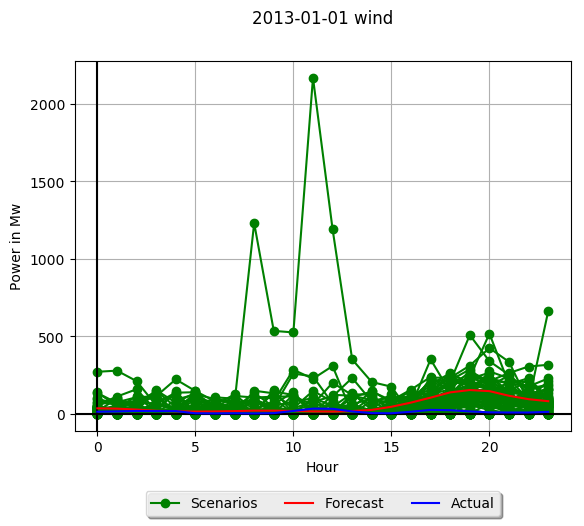
\includegraphics{wind.png}
	\end{figure}	
	
\end{document}